As discussed in the previous section, no article has been found on dual-evaporator transcritical
HTHP's.  However, a short liretature review on the current state of the art technology for HTHP's
has been conducted and lead to the identification of several reasons why the topic could potentially be 
of particular interest. \\

First, on the dual-evaporator.  It is shown in \cite{mateu2021advanced} that the use of 
multiple evaporators has a significant potential for waste heat recovery applications.
In the study case considered, they observed significant improvements in Coefficient of Performance (COP)
and Volumetric Heating Capacity (VHC) when using two evaporators instead of one as soon as a significant
portion of the heat was available at the medium temperature level (MT) (see Figure \ref{fig:mateu2021advanced}).
This heat source ratio parameter was first introduced in \cite{arpagaus2016multi} as the $\beta$ parameter:
$$\beta \triangleq \frac{\dot{Q}_{MT}}{\dot{Q}_{MT} + \dot{Q}_{LT}}$$
where $\dot{Q}_{MT}$ and $\dot{Q}_{LT}$ are the thermal powers rates captured at the medium and low temperature evaporators.


\begin{figure}[H]
    \centering
    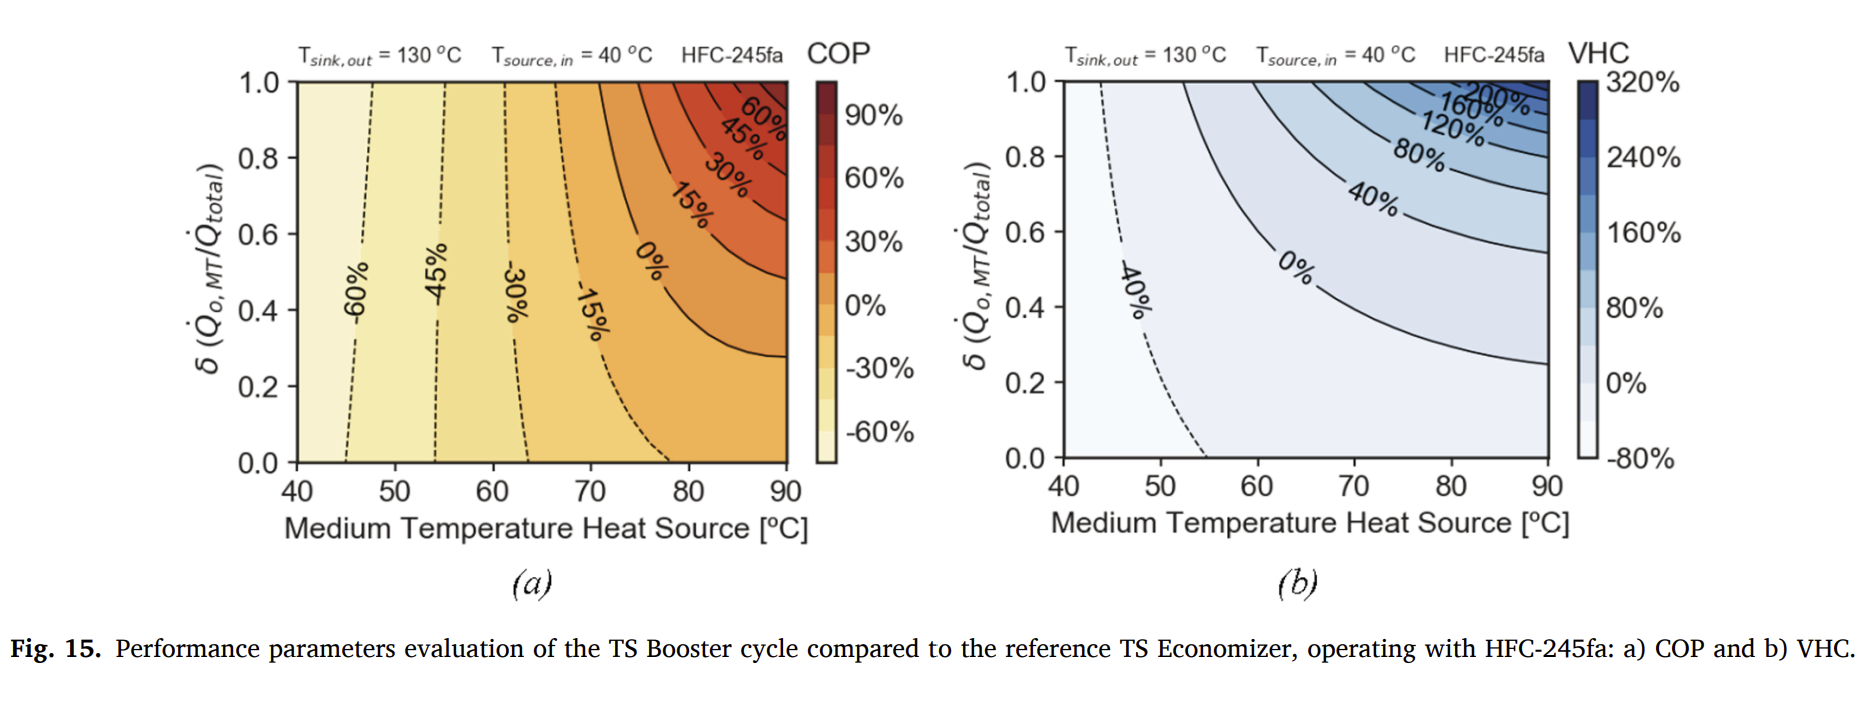
\includegraphics[width=\textwidth]{Figures/COP_and_VHC_improvement.png}
    \begin{minipage}{0.9\textwidth}
    \caption{The COP and VHC improves drastically when using two evaporators instead of one as soon as the portion
    of heat captured at the medium temperature source accounts for a significant part of the total heat captured.
    Figure taken from \cite{mateu2021advanced}.}
    \label{fig:mateu2021advanced}
    \end{minipage}
\end{figure}

\noindent The intrest of having a higher COP is not to be demonstrated.  However, the VHC value is also of 
particular interest since, as explained in \cite{arpagaus2018high}, it is directly linked to the size of the compressor.
The higher the VHC, the smaller the refrigerant charge and compressor, reducing the cost of the system. \\

Then, on the transcritical aspect of the cycle.  In \cite{vieren2023thermodynamic}, the authors show that
the use of a transcritical cycle instead of a subcritical one can lead to significant improvements in the COP
when the temperature glide at the heat sink is high.  According to them, the ideal heat sink temperature
glide is around 60 K.  This COP increase is explained by a lower temperature mismatch during the heat transfer 
at the heat sink (see Figure \ref{fig:temperature_mismatch}).  This improved temperature matching is due to
the properties of a supercritical fluid.  Indeed since the heat transfer occurs above the critical pressure,
the fluid does not undergo a phase change.  Therefore, its temperature can vary significantly during the heat transfer,
leading to a better temperature matching with the heat sink fluid.   

\begin{figure}[H]
    \centering
    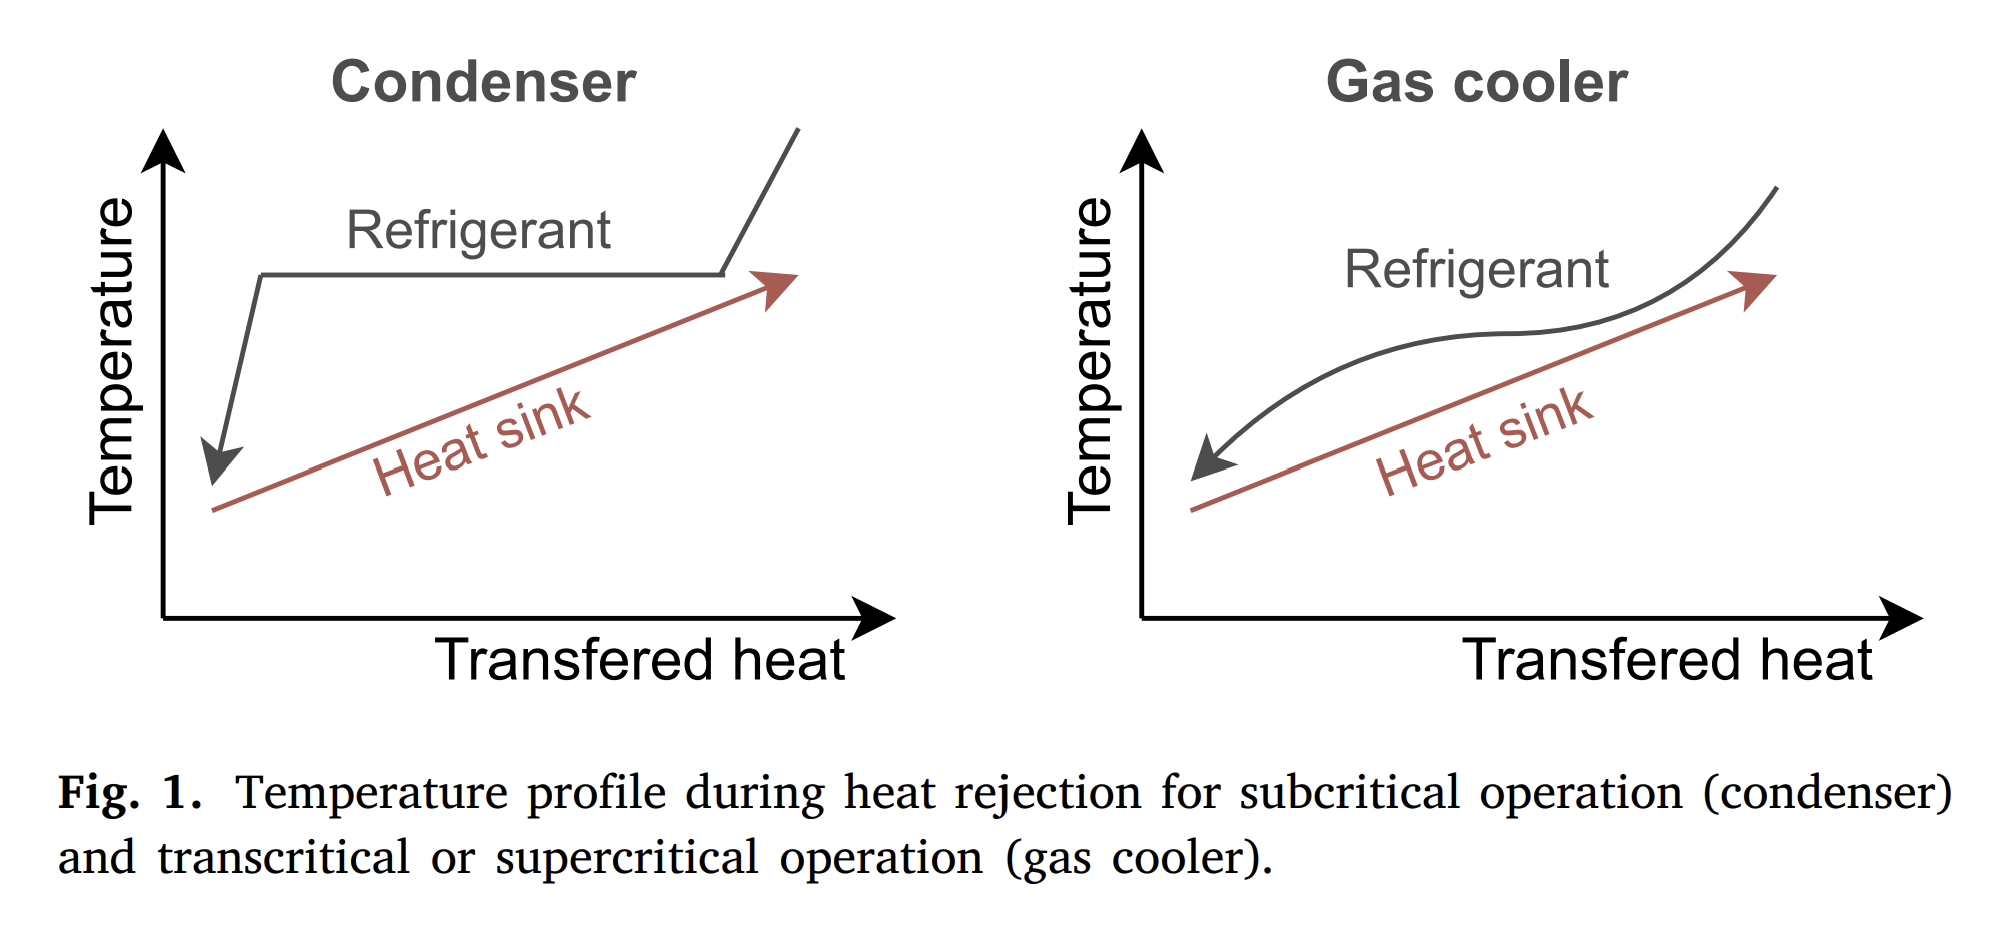
\includegraphics[width=0.8\textwidth]{Figures/Heat_transfer_improvement.png}
    \begin{minipage}{0.9\textwidth}
    \caption{The area between the two curves represents the exergy destruction due to the heat transfer.
    This area is significantly lower in the transcritical case, leading to reduced irreversibilities and potentially 
    leading to a higher COP.  Figure taken from \cite{vieren2023thermodynamic}.}
    \label{fig:temperature_mismatch}
    \end{minipage}
\end{figure}

\noindent Additionally, in \cite{vieren2023thermodynamic}, the authors show that transcritical cycles 
generally lead to higher VHC values than subcritical ones. \\

Finally, on the high temperature. \\

\textcolor{red}{To be completed by FG (2 pages).}

As a conclusion, a dual-evaporator transcritical high temperature heat pump could potentially
show higher performance than current HTHP's on the market in applications where heat is available at
two temperature levels (e.g. waste heat recovery) and where the temperature glide at the heat sink is high.